\documentclass{article}
\usepackage[margin=1in]{geometry}
\usepackage{longtable,graphicx}
\begin{document}
\section*{Six-flow source recovery evaluation}
PASS means no reproducible final divergence was detected within the recorded valid inputs and budget; it is not a universal equivalence proof.
\begin{longtable}{llllllllllllllll}
Flow & N & Eligible N & First-pass RSR & Final RSR@R & Program Behavioral Pass Rate & Initial Behavioral Pass Rate & Final Behavioral Pass Rate & Input Match Macro & Input Match Micro & Counterexample Detection Rate & Re-executability Rate & Compilation Repair Gain & Behavioral Repair Gain & Mean Tokens & Mean Runtime \\ \hline
F1 & 40 & 40 & 37/37 (100.0\%) & 37/37 (100.0\%) & 36/37 (97.3\%) & 27/37 (73.0\%) & 36/37 (97.3\%) & 97.3\% & 100.0\% & 1/37 (2.7\%) & 37/40 (92.5\%) & +0.0 pp & +24.3 pp & 467513 & 169.5s \\
F2 & 40 & 40 & 30/31 (96.8\%) & 30/31 (96.8\%) & 21/30 (70.0\%) & 21/30 (70.0\%) & 21/30 (70.0\%) & 90.7\% & 95.8\% & 9/30 (30.0\%) & 30/40 (75.0\%) & N/A & N/A & 158288 & 75.7s \\
F3 & 40 & 40 & 37/37 (100.0\%) & 37/37 (100.0\%) & 36/37 (97.3\%) & 25/37 (67.6\%) & 36/37 (97.3\%) & 97.3\% & 100.0\% & 1/37 (2.7\%) & 37/40 (92.5\%) & +0.0 pp & +29.7 pp & 279570 & 143.0s \\
F4 & 40 & 40 & 39/40 (97.5\%) & 40/40 (100.0\%) & 36/40 (90.0\%) & 21/40 (52.5\%) & 36/40 (90.0\%) & 96.9\% & 99.4\% & 4/40 (10.0\%) & 40/40 (100.0\%) & +2.5 pp & +37.5 pp & 237525 & 176.5s \\
F5 & 40 & 40 & 36/38 (94.7\%) & 38/38 (100.0\%) & 24/38 (63.2\%) & 14/38 (36.8\%) & 24/38 (63.2\%) & 70.3\% & 82.6\% & 14/38 (36.8\%) & 38/40 (95.0\%) & +5.3 pp & +26.3 pp & 1154891 & 293.3s \\
F6 & 40 & 40 & 23/23 (100.0\%) & 23/23 (100.0\%) & 11/23 (47.8\%) & 11/23 (47.8\%) & 11/23 (47.8\%) & 63.2\% & 66.0\% & 12/23 (52.2\%) & 23/40 (57.5\%) & N/A & N/A & 367079 & N/A \\
\end{longtable}
\section*{Source quality: accepted Recovered C Source only}
Readability is an independent 1-to-5 assessment of Variables, Loops, Conditions, Logic flow, and Structural integrity. It is not a correctness metric.
\begin{longtable}{llllllllll}
Flow & Accepted & Evaluated & Coverage & Variables & Loops & Conditions & Logic flow & Structural integrity & Overall \\ \hline
F1 & 36 & 36 & 36/36 (100.0\%) & 2.94 & 3.86 & 3.61 & 3.78 & 3.58 & 3.56 \\
F2 & 21 & 21 & 21/21 (100.0\%) & 2.71 & 3.95 & 3.48 & 3.81 & 3.67 & 3.52 \\
F3 & 36 & 36 & 36/36 (100.0\%) & 3.53 & 4.14 & 3.97 & 4.19 & 4.06 & 3.98 \\
F4 & 36 & 36 & 36/36 (100.0\%) & 2.81 & 3.86 & 3.56 & 3.86 & 3.64 & 3.54 \\
F5 & 24 & 24 & 24/24 (100.0\%) & 3.83 & 4.46 & 4.38 & 4.50 & 4.38 & 4.31 \\
F6 & 11 & 11 & 11/11 (100.0\%) & 4.00 & 4.73 & 4.64 & 4.73 & 4.64 & 4.55 \\
\end{longtable}
\begin{figure}[p]\centering
\includegraphics[width=.9\linewidth]{figures/overall_performance.pdf}\caption{Primary recovery outcomes with executable availability over all eligible samples; F6 is derived from F5's first provider call.}\end{figure}
\begin{figure}[p]\centering
\includegraphics[width=.9\linewidth]{figures/compilation_performance.pdf}\caption{Compilation success before and after repair.}\end{figure}
\begin{figure}[p]\centering
\includegraphics[width=.9\linewidth]{figures/behavioral_performance.pdf}\caption{Behavioral outcomes over conclusive campaigns.}\end{figure}
\begin{figure}[p]\centering
\includegraphics[width=.9\linewidth]{figures/repair_effectiveness.pdf}\caption{Behavioral repair effectiveness; F2, F6 repair fields are N/A.}\end{figure}
\begin{figure}[p]\centering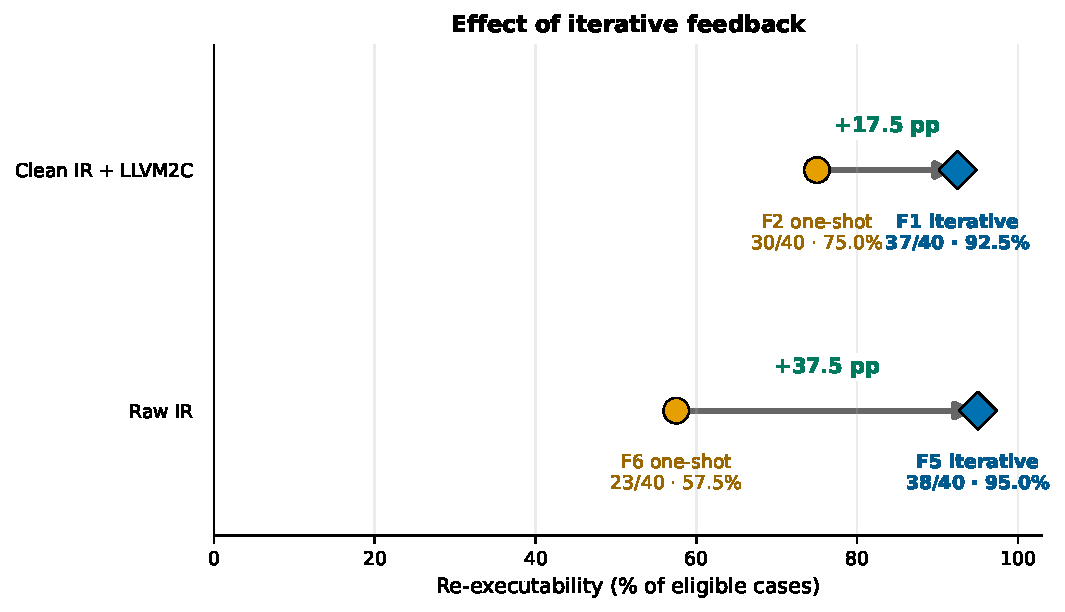
\includegraphics[width=.9\linewidth]{figures/iterative_feedback_vs_one_shot.pdf}\caption{Matched-evidence re-executability comparison of iterative feedback against one-shot reconstruction.}\end{figure}
\begin{figure}[p]\centering
\includegraphics[width=.9\linewidth]{figures/cumulative_compile_success_by_round.pdf}\caption{Cumulative executable creation by compile attempt.}\end{figure}
\begin{figure}[p]\centering
\includegraphics[width=.9\linewidth]{figures/cumulative_behavioral_success_by_round.pdf}\caption{Cumulative behavioral pass by campaign.}\end{figure}
\begin{figure}[p]\centering
\includegraphics[width=.9\linewidth]{figures/final_status_breakdown.pdf}\caption{Final status distribution without collapsing INCONCLUSIVE into failure.}\end{figure}
\begin{figure}[p]\centering
\includegraphics[width=.9\linewidth]{figures/failure_taxonomy.pdf}\caption{Compilation, behavioral, and inconclusive taxonomies.}\end{figure}
\begin{figure}[p]\centering
\includegraphics[width=.9\linewidth]{figures/sample_flow_status_heatmap.pdf}\caption{0=fail, 1=unresolved, 2=pass by paired sample and flow.}\end{figure}
\begin{figure}[p]\centering
\includegraphics[width=.9\linewidth]{figures/sample_flow_match_heatmap.pdf}\caption{Input match (\%) by paired sample and flow.}\end{figure}
\begin{figure}[p]\centering
\includegraphics[width=.9\linewidth]{figures/ablation_forest_plot.pdf}\caption{Paired re-executability effects with bootstrap 95\% CI.}\end{figure}
\begin{figure}[p]\centering
\includegraphics[width=.9\linewidth]{figures/ablation_win_tie_loss.pdf}\caption{Paired win/tie/loss counts for re-executability.}\end{figure}
\begin{figure}[p]\centering
\includegraphics[width=.9\linewidth]{figures/tokens_vs_e2e.pdf}\caption{Total tokens versus Re-executability outcome.}\end{figure}
\begin{figure}[p]\centering
\includegraphics[width=.9\linewidth]{figures/runtime_vs_behavioral_pass.pdf}\caption{Runtime (seconds) versus Behavioral pass outcome.}\end{figure}
\begin{figure}[p]\centering
\includegraphics[width=.9\linewidth]{figures/llvm_reduction_summary.pdf}\caption{LLVM simplification metrics; these are not correctness claims.}\end{figure}
\begin{figure}[p]\centering
\includegraphics[width=.9\linewidth]{figures/llvm_reduction_vs_behavior.pdf}\caption{Association view only; LLVM reduction is not a semantic oracle.}\end{figure}
\begin{figure}[p]\centering
\includegraphics[width=.9\linewidth]{figures/stage_completion_funnel.pdf}\caption{Stage completion rates with explicit numerators and denominators in the report.}\end{figure}
\end{document}
